\documentclass{iau} 
\usepackage{graphicx}
\usepackage{natbib}
\usepackage{hyperref}
%\usepackage{doi}

\pubyear{2022}
\volume{372}
\setcounter{page}{1}
\jname{The Era of Multi-Messenger Solar Physics}
\editors{G.~Cauzzi \& A.~Tritschler, eds.}

\title[Hot Chromospheric Fibrils] %% give here short title %%
{Spatio-temporal Characterization of Hot Chromospheric Fibrils}

\author[Lamb et al.]   %% give here short author list %%
{Parker Lamb$^{1,2}$, Gianna Cauzzi$^{1,3}$ \and Kevin Reardon$^{1,4}$}

\affiliation{$^1$National Solar Observatory, Boulder, CO 80303, USA \\ [\affilskip]
$^2$Department of Physics, University of Colorado, Boulder, CO 80309, USA \\ [\affilskip]
$^3$INAF -- Osservatorio Astrofisico di Arcetri, 50125 Firenze, Italy \\ [\affilskip]
$^4$Department of Astrophysics and Planetary Sciences, University of Colorado, Boulder, CO 80303, USA}


\begin{document}

\maketitle

\begin{abstract}
The exact mechanisms leading to chromospheric heating are still ill-defined. While the presence of magnetic elements is undoubtedly necessary, the details of the heating, and its spatio-temporal distribution remain poorly understood. 
We contribute to this topic by analyzing the behavior of hot chromospheric fibrils surrounding network and plage elements, identified via the broader H$\alpha$ profiles observed along their length, as the H-$\alpha$ spectral line width has been shown to correlate with the local chromospheric temperatures through comparison with the ALMA millimeter-continuum brightness temperature. We make use of loop tracing and analysis software to investigate characteristics of the chromospheric hot fibrils
including their length, number density, and transverse spatial extension in an enhanced network region, and provide measurements on their temporal evolution. 

\keywords{Sun: chromosphere, Sun: faculae, plage}
\end{abstract}

%\firstsection % if your document starts with a section, you can
              % remove some space above using this command.
              
\section{Introduction}
%The text of your contribution starts here. You can use the $\backslash$cite command like this: 
%\cite{2009A&A...503..577C,2015HiA....16..439C}. A sample figure is shown below.

A clear explanation of the mechanisms leading to heating of the solar chromosphere still eludes us. The energy requirements are significant: on average, the chromosphere radiates 4 kWm$^{-2}$ in quiet Sun, and 20 kWm$^{-2}$ in active regions, as derived from the earlier work of \citet{1977ARA&A..15..363W} and \citet{1981ApJS...45..635V}. However, recent studies based on high resolution observations point to sensibly higher values, at least in some portions of plage and active regions \citep[up to 90 and 160 kWm$^{-2}$ respectively, see][]{2022A&A...664A...8M, 2021A&A...647A.188D}.

We know that the presence of magnetic elements is an important factor: beside active regions, both quiet Sun and plage regions show increased emission 
in areas where strong (photospheric) fields are present. The role of chromospheric magnetic fields has also recently become a subject of study, with \citet{2018A&A...612A..28L} finding that enhanced radiative losses are correlated with the strength of the horizontal chromospheric fields. In general, however, analyses of the spatio-temporal distribution of chromospheric heating are still sparse, as they require high spatial and temporal resolution, long-duration observations
as well as significant spectral and polarimetric information to derive the thermodynamical and magnetic properties of the atmosphere \citep[see e.g. the recent study by][]{2022A&A...664A...8M}. 

%Morosin et al 2022 have vey nice data & analysis. Q and U in CaII 8542 however are still too noisy to use. Maybe we can do better with the DDT data?
% they talk about the "bottom edge of the hot canopy" as seen from T maps obtained in CaII 8542 - the fibrils we discuss could easily be the same thing. BUT,
% they claim that hydrogen is the biggest contributor in the highest part of the chromosphere (sort of confirmed when comparing with ALMA), so maybe that
% is what we look at. Hydrogen is the biggest contributor. They derive Temperatures of max 9.5 kK
% They look for a periodicity in the radiative term, which is most likely due to magnetoacoustic shocks - they find a period of ~ 5 min - in line with the idea of
% p modes penetrating the higher parts of the atmosphere, but the amplitude is ~ 30% of the total loss. The "non periodic" part is not looked at much - it could be 
% changing at time steps less than their cadence (35 s) for example, and in any case it still retains the fairly "fingery" appearance of the hot fibrils we discuss here. 
%Even if they say that it is "smooth", I do not see that! But it might be that it is so fast that we see it constant - check Cauzzi et al 2009, Rutten discussions etc
% keep in mind, de la Cruz Rodr’guez, J., De Pontieu, B., Carlsson, M., & Rouppe van der Voort, L. H. M. 2013, ApJ, 764, L11

A constant characteristics of areas of concentrated magnetic elements such as network or plage regions, is the presence of a multitude of fibrilar strutcures, anchored
in the strong magnetic elements at the photosphere, as usually observed in the core of strong chromospheric spectral lines. These have been long observed for
example
using the H$\alpha$ line, and variously dubbed as  ``mottles", ``rosettes'', or spicules \citep[][among many]{1968SoPh....3..367B, 2006ASPC..354..276R,2012SSRv..169..181T}. 
% and repres slender fibrils stuff in CaII K, see Rutten 2005 etc). Many doubts still remain about their origin and physical properties: for example they are usually assumed to outline the direction of the chromospheric magnetic field, but ... (Schad et al. Any new work?). Some of the bigger fibrils  are nicely
%identified as due to periodic magneto-acoustic shocks developing at
%chromospheric levels (``dynamic fibrils", or type-I spicules, see Hansteen 2006; someone else), while others, much more slender, are often classified as type-II spicules (De Pontieu...) and apparently harbor strong 
%upward motions induced by explosive reconnection ...(De pontieu again, Rouppe etc). 
%might appear almost instantaneously and display large swaying motions betraying Alfven waves (??? some De Pontieu for sure).
%We note however that at least some of these features might appear as "optical illusions", 
%due the temporary overlap of optically thin plasma suspended in swaying current sheets .... (Judge et al 2012).
Their origin is still somewhat debated, but the important consideration for our present study is that such fibrils seem to be the site of strong heating events. This was originally recognized by \citet{2009A&A...503..577C},
who showed how the immediate surroundings of network and plage elements would correspond to volumes of plasma hotter than the average, as indicated by the enhanced values of the spectral line widths of both H$\alpha$ and the CaII 854.2 nm line. This finding was put on firmer footing 
by \citet{2019ApJ...881...99M}, that clearly demonstrated how regions of enhanced H$\alpha$ spectral width coincide with area of high brightness temperature as inferred from the ALMA millimeter-continuum emission  (T$_b$, which
corresponds to the electronic temperature, T$_e$). The recent work of \citet{2023FrASS...9.8405T} further confirmed this correspondence.

Given the likely relevance of these ``hot chromospheric fibrils'' in the general problem of chromospheric heating, we have initiated a study of their quantitative characteristics, with the final objective of constraining possible heating mechanisms in this mysterious part of the solar atmosphere.  

\section{Analysis and results}\label{sec_data}

The relevant data was acquired with the Interferometric Bidimensional Spectrometer \citep[IBIS,][]{2006SoPh..236..415C} on April 23, 2017, and included sampling of the 
chromospheric lines H$\alpha$,
NaI D$_1$ and CaII 854.2 nm in multiple wavelengths per line, with a cadence of $\sim$16 s over a total of 46 minutes  \citep[note that this is the same dataset analyzed in][]{2019ApJ...881...99M,2022ApJ...933..244H}. The 96'' $\times$ 96'' field of view (FOV) covered a stable plage area in the vicinity of an active region, as shown in the left panel of Figure \ref{fig_fov}, taken in the core of H$\alpha$.  The right panel of
Figure  \ref{fig_fov} shows instead the map of H$\alpha$ spectral width, calculated from the whole spectral line as described in \citet{2009A&A...503..577C}. A multitude of hot fibrils are clearly seen, jutting out of the plage magnetic elements. While the general orientation of the fibrilar features is the same in the two panels, note that hot fibrils (i.e. bright features in the map of H$\alpha$ spectral width) can coincide with features that are either bright or dark in the intensity image. Moreover, the hot fibrils extend only for a certain fraction of the intensity fibrils, and do not cover the whole FOV.  

\begin{figure}[h]
\begin{center}
 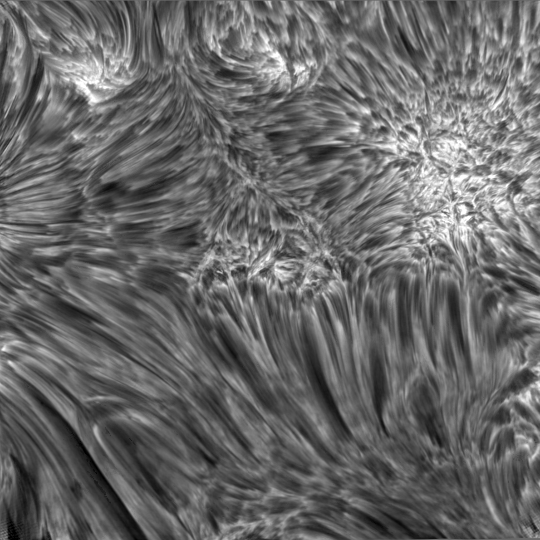
\includegraphics[width=0.4\textwidth]{fov.int.png} 
 \hspace{0.8cm}
  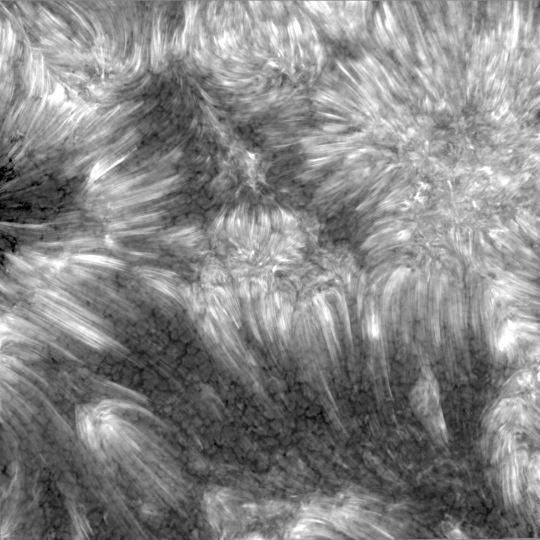
\includegraphics[width=0.4\textwidth]{fov.width.png} 
 \caption{Left: H$\alpha$ line core intensity in the analyzed plage area. The FOV is 96'' $\times$ 96'' (about 70 $\times$ 70 Mm). Right: Map of corresponding H$\alpha$
 spectral width. Values are scaled between 0.9 and 1.2 \AA, which correspond roughly to T$_b$ of 6-12,000 K, as per \citet{2019ApJ...881...99M}.}\label{fig_fov}
\end{center}
\end{figure}

The preliminary analysis described in this paper was conducted on a single map of H$\alpha$ width, obtained at a time of excellent seeing. We first performed a manual identification of the hot fibrils, using a high-pass difference image obtained by subtracting a Gaussian-smoothed width map from the original image, for easier tracing of small-scale features (Fig. \ref{fig_fibrils} left panel). The identification was performed multiple times, by multiple independent observers, to obtain 
a control set (Fig. \ref{fig_fibrils} center panel). Finally, we used the OCCULT-2 algorithm \citep{2013Entrp..15.3007A}, which identifies curvilinear features from an intensity image and outputs a table of feature coordinates, to perform an automatic tracing of the hot fibrils. OCCULT-2 was first designed to trace coronal loops in images with lower spatial resolution, but we optimized its parameters using the control set defined above to guide our choices. The resulting traces are shown in 
Fig. \ref{fig_fibrils} right panel. We identified a total of 515 fibrils in our 96'' $\times$ 96'' FOV.

\begin{figure}[h]
\begin{center}
%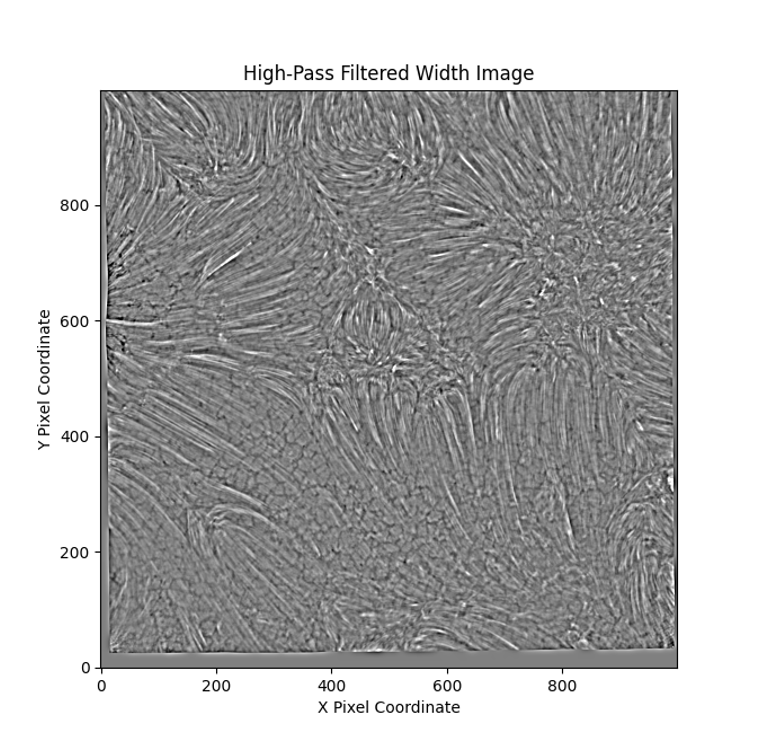
\includegraphics[width=0.3\textwidth]{highpass.png} 
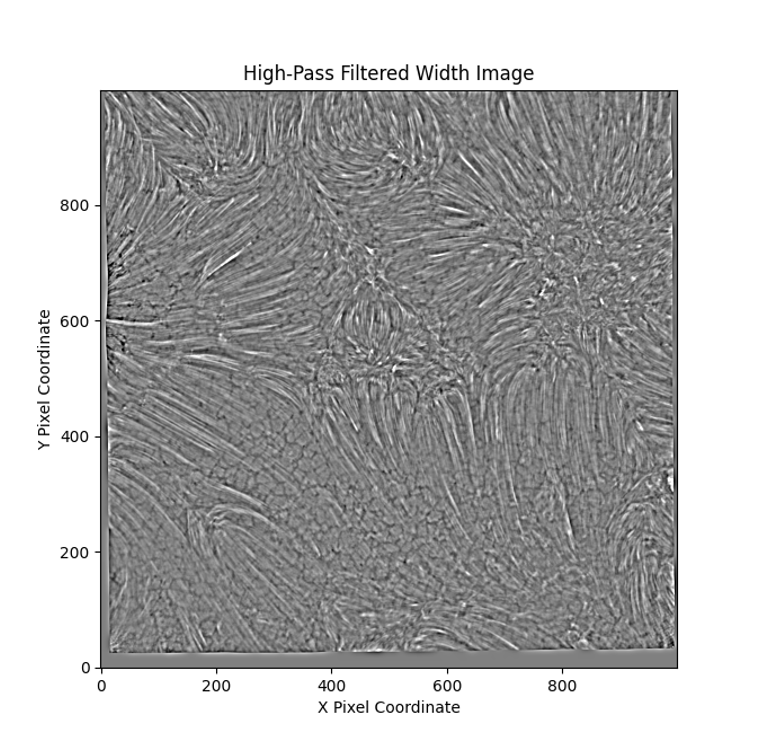
\includegraphics[width=4cm]{highpass.png} 
% \hspace{0.05cm}
% 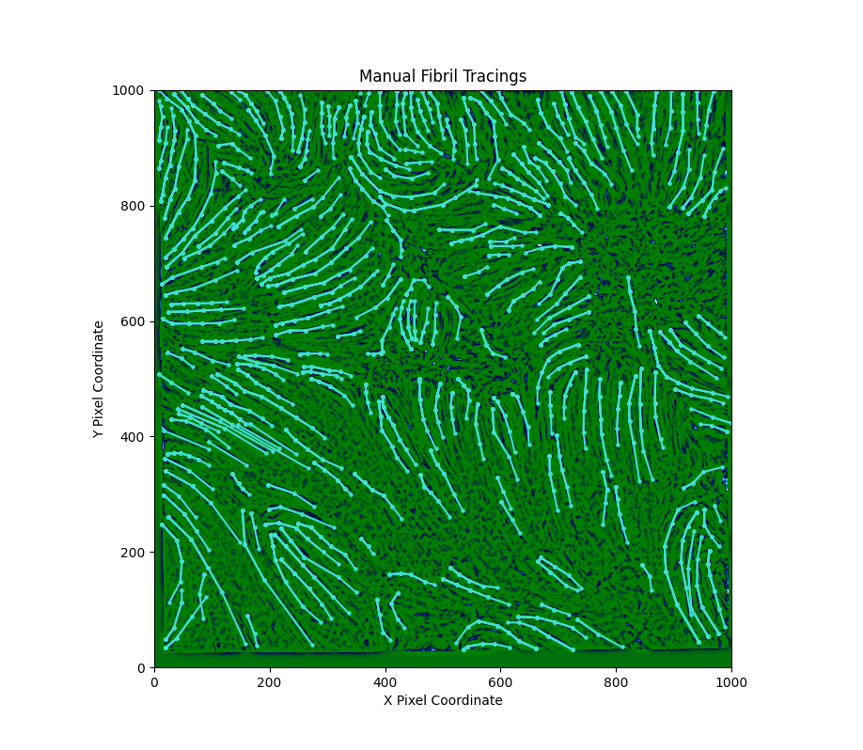
\includegraphics[width=0.34\textwidth]{manual.png} 
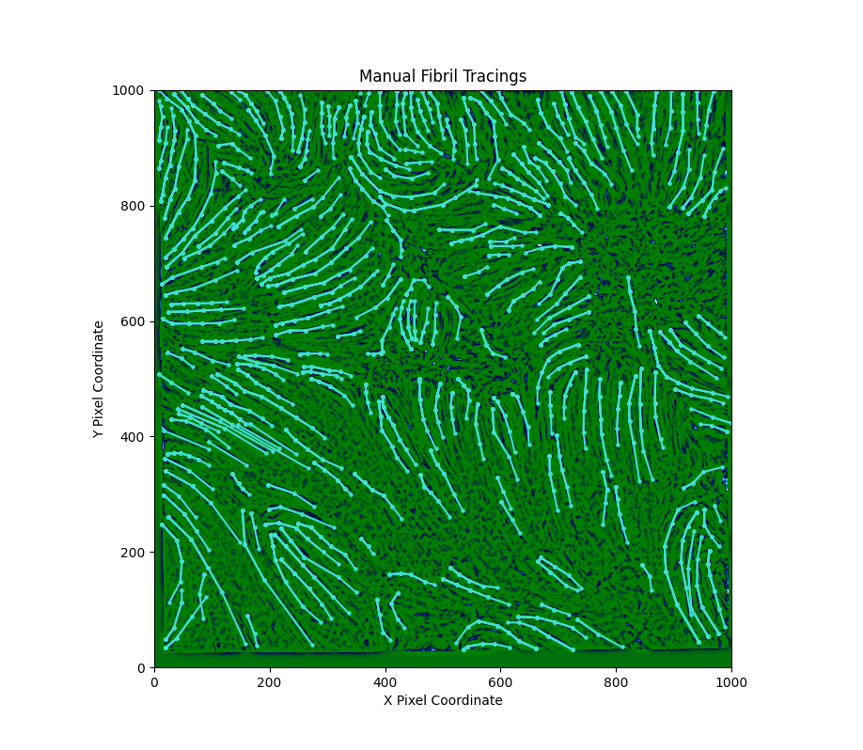
\includegraphics[width=4.53cm]{manual.png} 
%\hspace{0.05cm}
%\vspace{1cm}
 %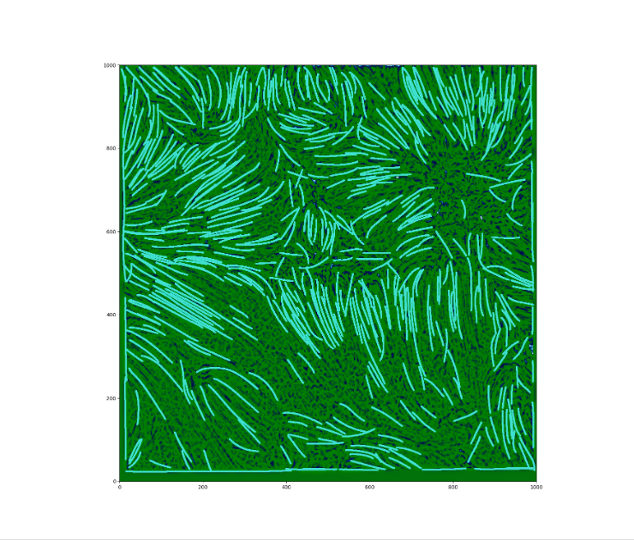
\includegraphics[width=0.35\textwidth]{occult.png} 
 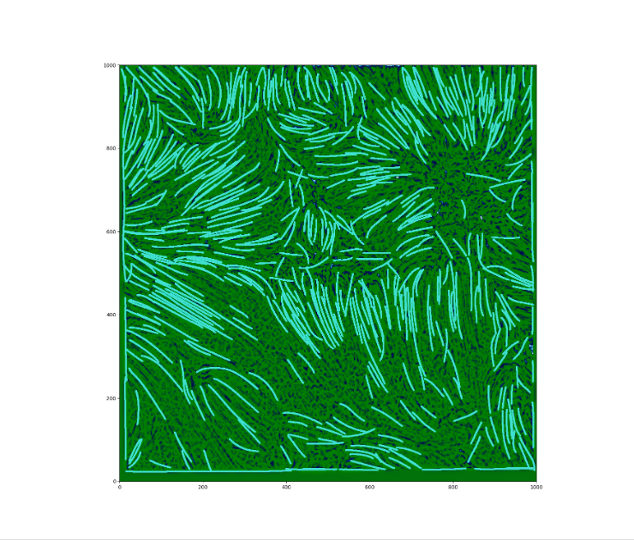
\includegraphics[width=4.57cm]{occult.png}  
 \caption{Left: High-pass difference image used to aid the manual identification of the hot fibrils. Center: Manual tracing (blue lines) of all visually-identifiable fibril lines in the width image (green background), for use as a control set. Right: Automatic tracing of fibrils by OCCULT-2 when using optimized parameters.} \label{fig_fibrils}
\end{center}
\end{figure}

Once we had the identified set of hot fibrils, we looked for three primary characteristics: length, spatial breadth and intensity. \textbf{Length} could be determined by summing up the Cartesian distances between each pixel along an identified fibril, such that, for a fibril composed of $n$ pixels, the length $L$ is
\begin{displaymath}
    L = \sum^n_{i=0} \sqrt{{\Delta x_n}^2+{\Delta y_n}^2}
\end{displaymath}

To calculate \textbf{breadth}, the spatial thickness of a fibril at any given point, we first detect "edges" in the images - contours along which where intensity changes sharply - using OpenCV's Canny edge detection algorithm based on \citet{1986CaJh}. Moving from pixel to pixel along the fibril, we look for the closest edge pixels on opposite sides of the fibril, then calculate the Cartesian differences between them. This method is visualized in \autoref{breadth_visualization}, and demonstrated in \autoref{canny_images} right panel. 

\begin{figure}[h]
    \begin{center}
    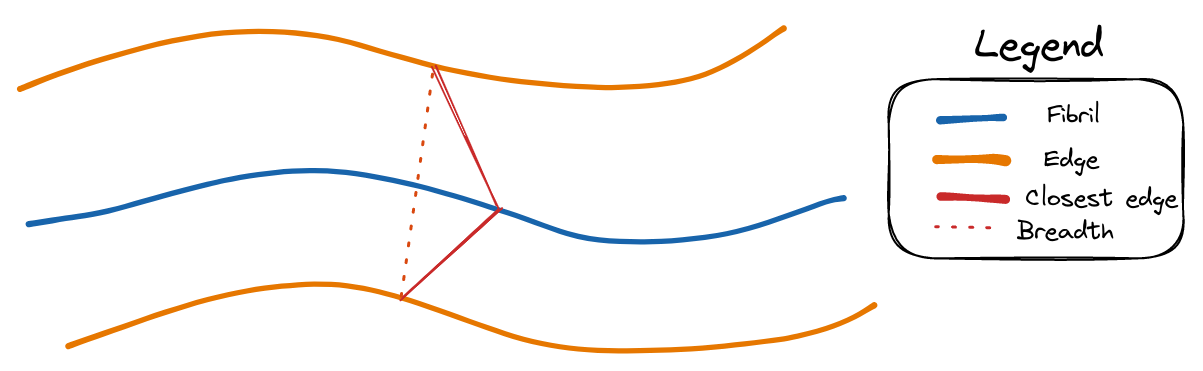
\includegraphics[width=7.5cm]{breadth_visualization.png} 
    % 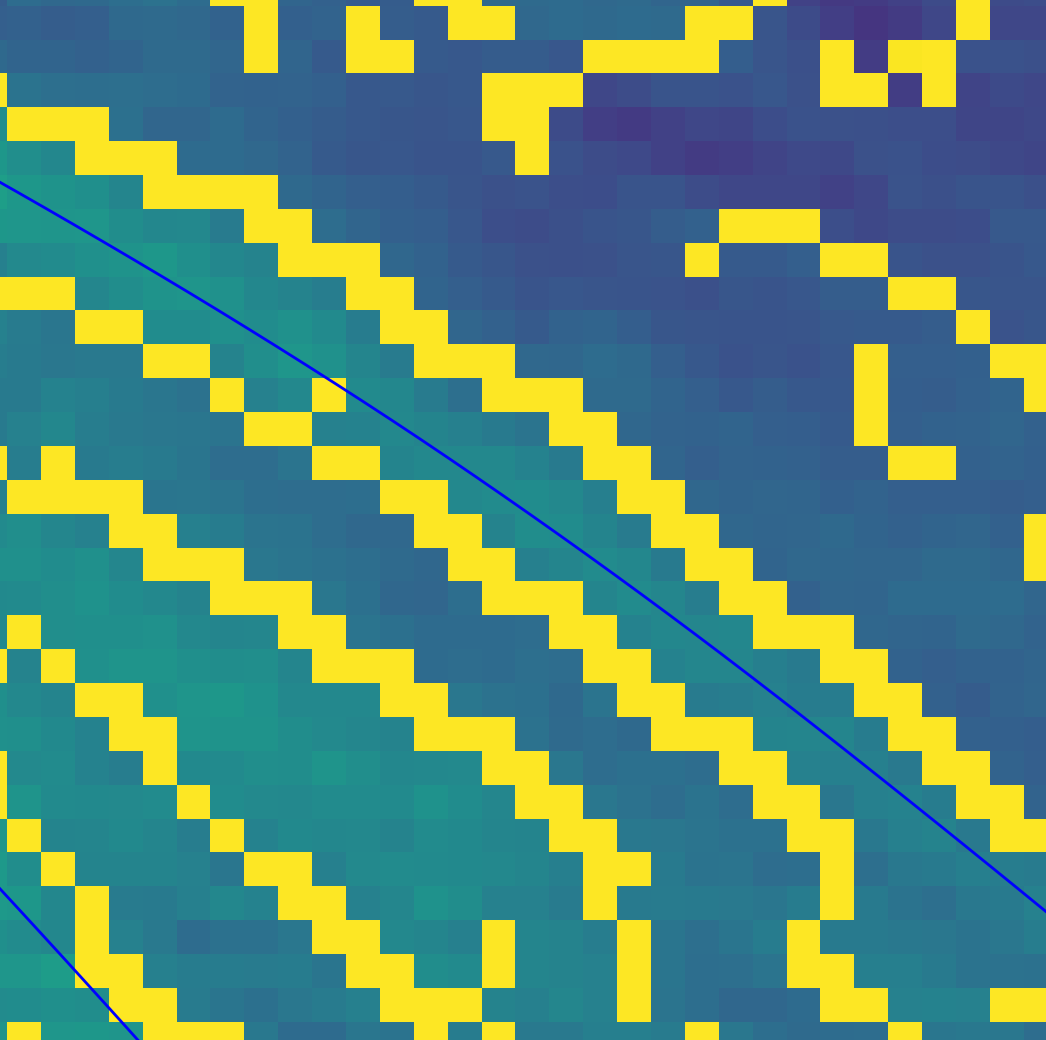
\includegraphics[width=4cm]{canny_edge_analysis.png} 
    %  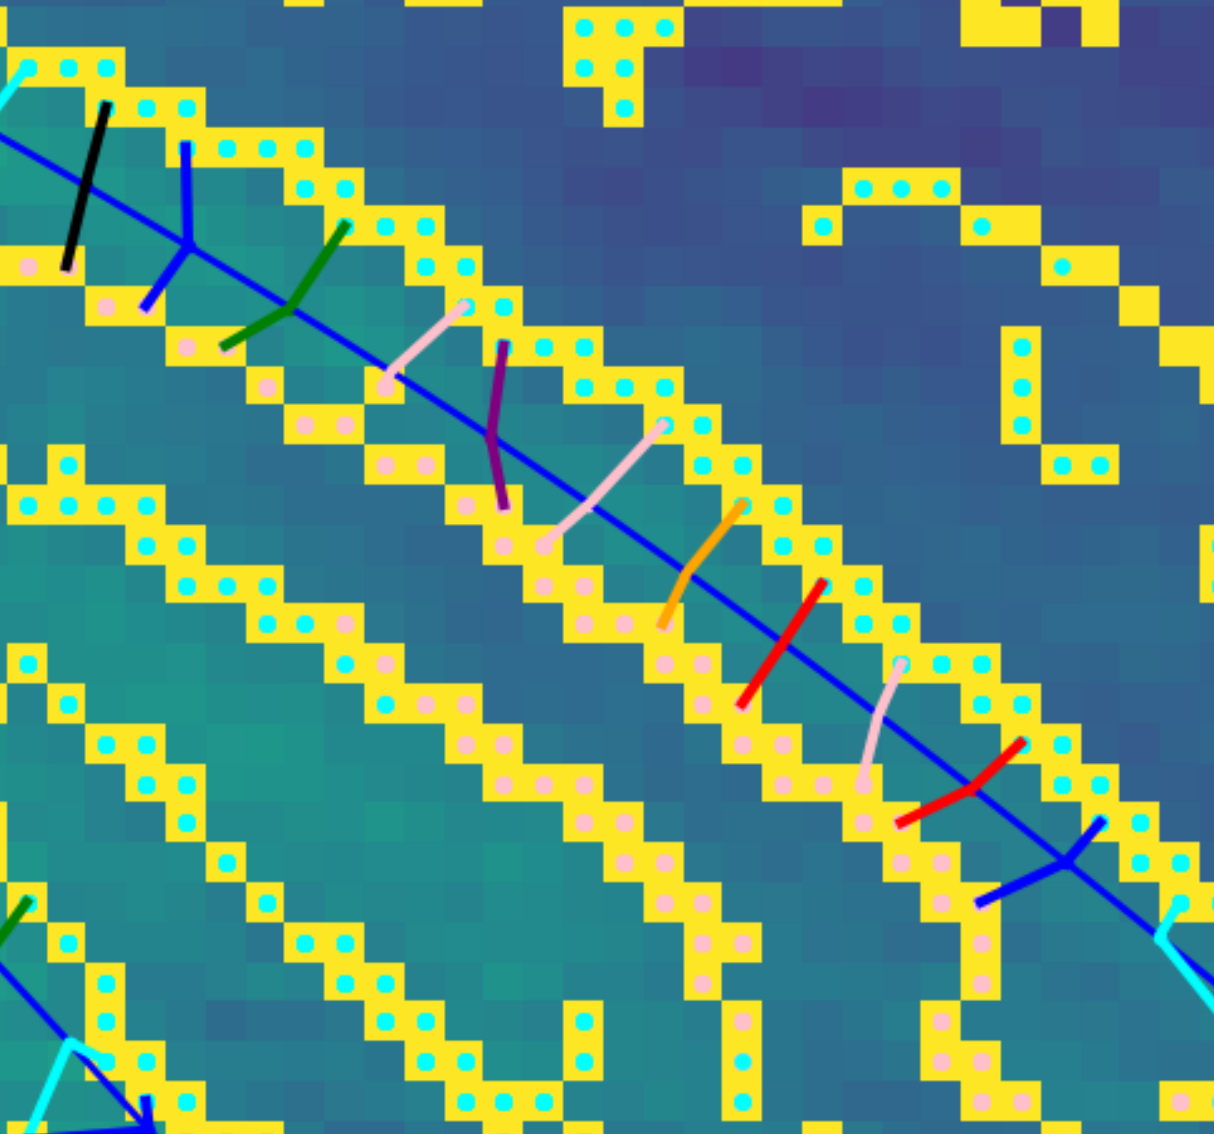
\includegraphics[width=4.3cm]{canny_edge_breadth.png}  
    \end{center}
    \caption{Demonstration of breadth calculation. The orange lines represent the detected edges, the blue the contained fibril, and red marks the path to the closest pixel on opposite sides. The dotted red line represents the calculated breadth.} \label{breadth_visualization}
\end{figure}

% How verbose to be about Canny's edge detection? Is this okay?

\begin{figure}[h]
    \begin{center}
    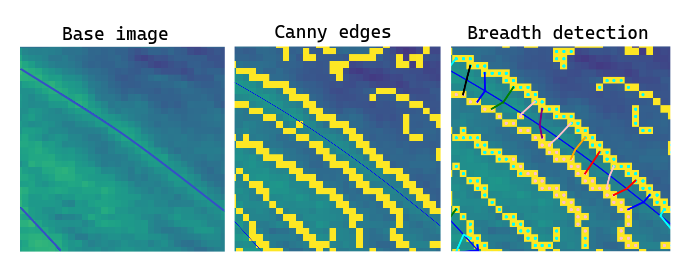
\includegraphics[width=12cm]{canny_section.png} 
    % 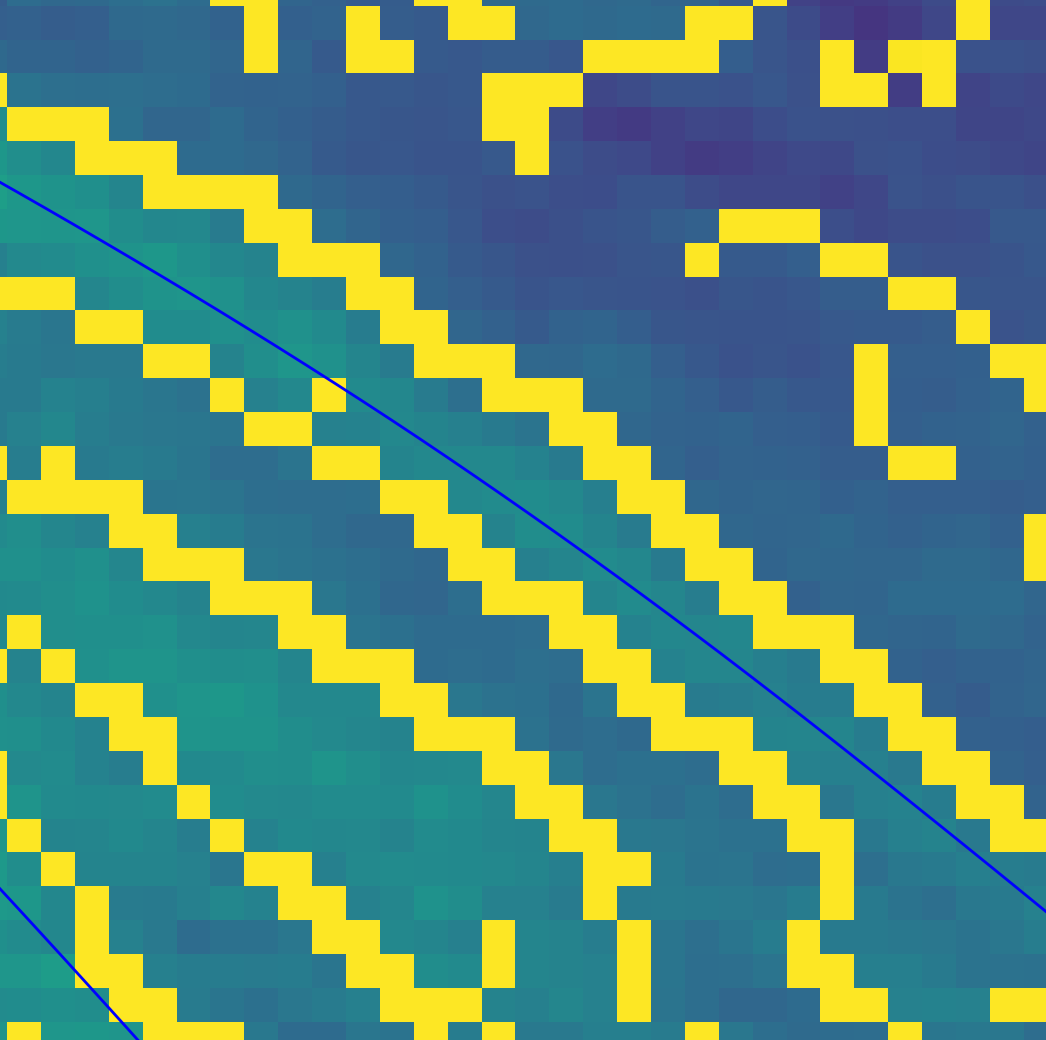
\includegraphics[width=4cm]{canny_edge_analysis.png} 
    %  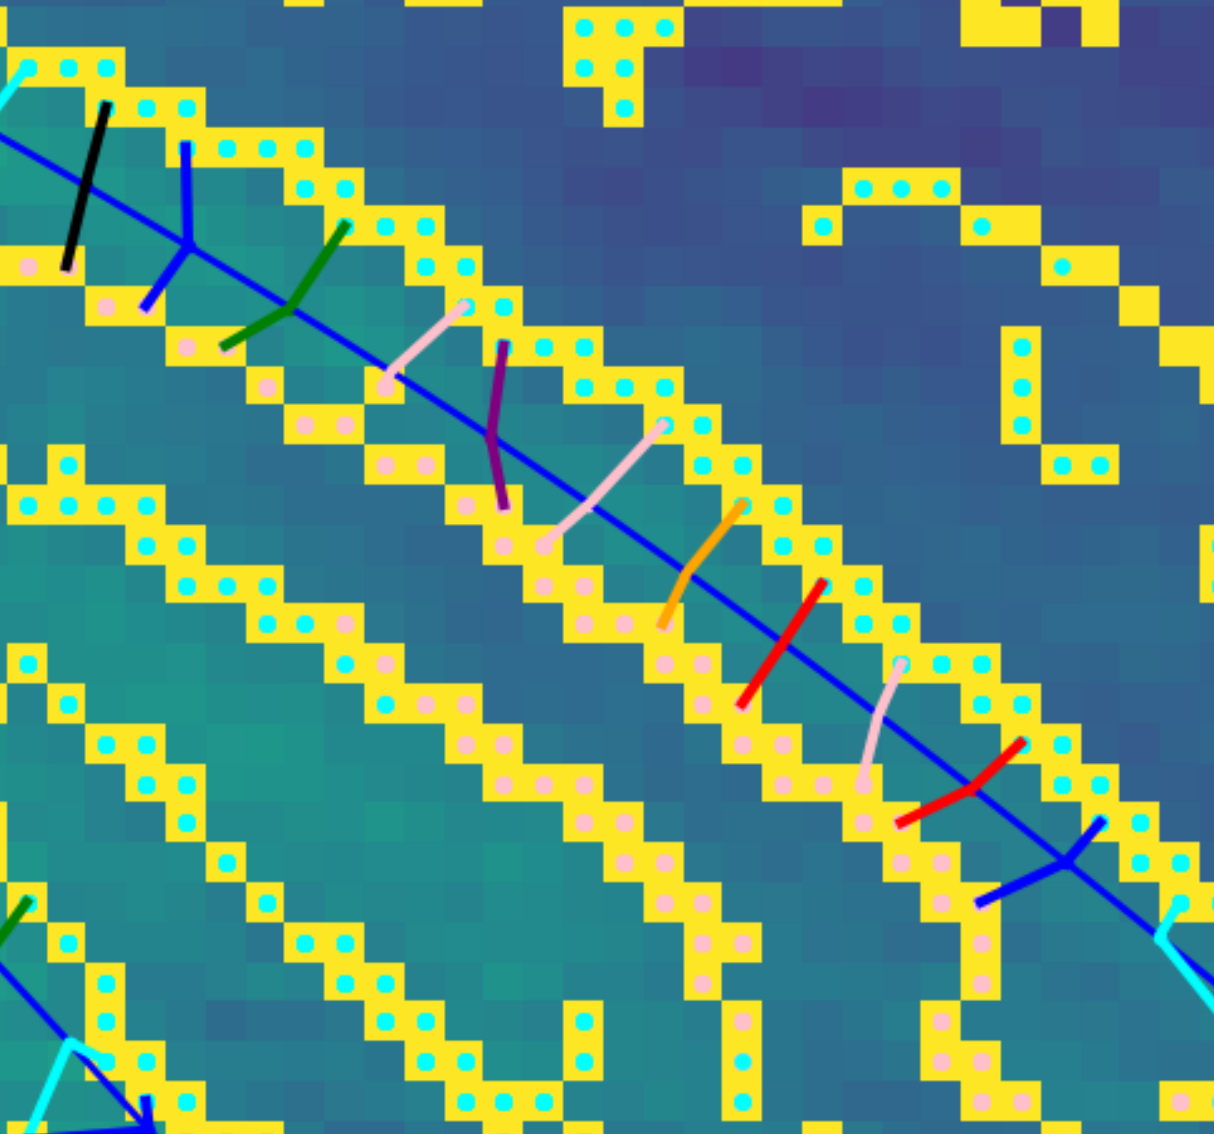
\includegraphics[width=4.3cm]{canny_edge_breadth.png}  
     \caption{Left: Base H$\alpha$ core width image used prior to Canny edge detection, cropped for demonstration purposes. Center: OpenCV's Canny edge detection algorithm applied to the base image. Right: per-pixel breadth estimation using detected edges.} \label{canny_images}
    \end{center}
\end{figure}

\textbf{Intensity} is the value of the H$\alpha$ spectral width at any given pixel along the length of the fibril - recorded primarily for comparisons with width and length to check for positive correlations on a per-pixel basis. 

The results are summarized in the histograms of \autoref{fig_results}. The hot fibrils display a large range of lengths (note that we adopted an arbitrary
 threshold of 2450 km, or 35 pixels on our image, as the minimum length to help with noise reduction), all the way to 10,000 km, with an average length of 5,500 km. Their average intensity, e.g. H$\alpha$ spectral width, is around 1.2 \AA, which is close to the upper limit reported in \citet{2019ApJ...881...99M}, and corresponds to a T$_e$ of over 10,000 K. Maybe most interesting, the breadth distribution shows that fibrils are very narrow, with values very close to the diffraction limit of the observations (2 pixels, or 150 km). This suggests that the mechanisms that lead to heating in these chromospheric features operate on very small spatial scales.

\begin{figure}[h]
\begin{center}
 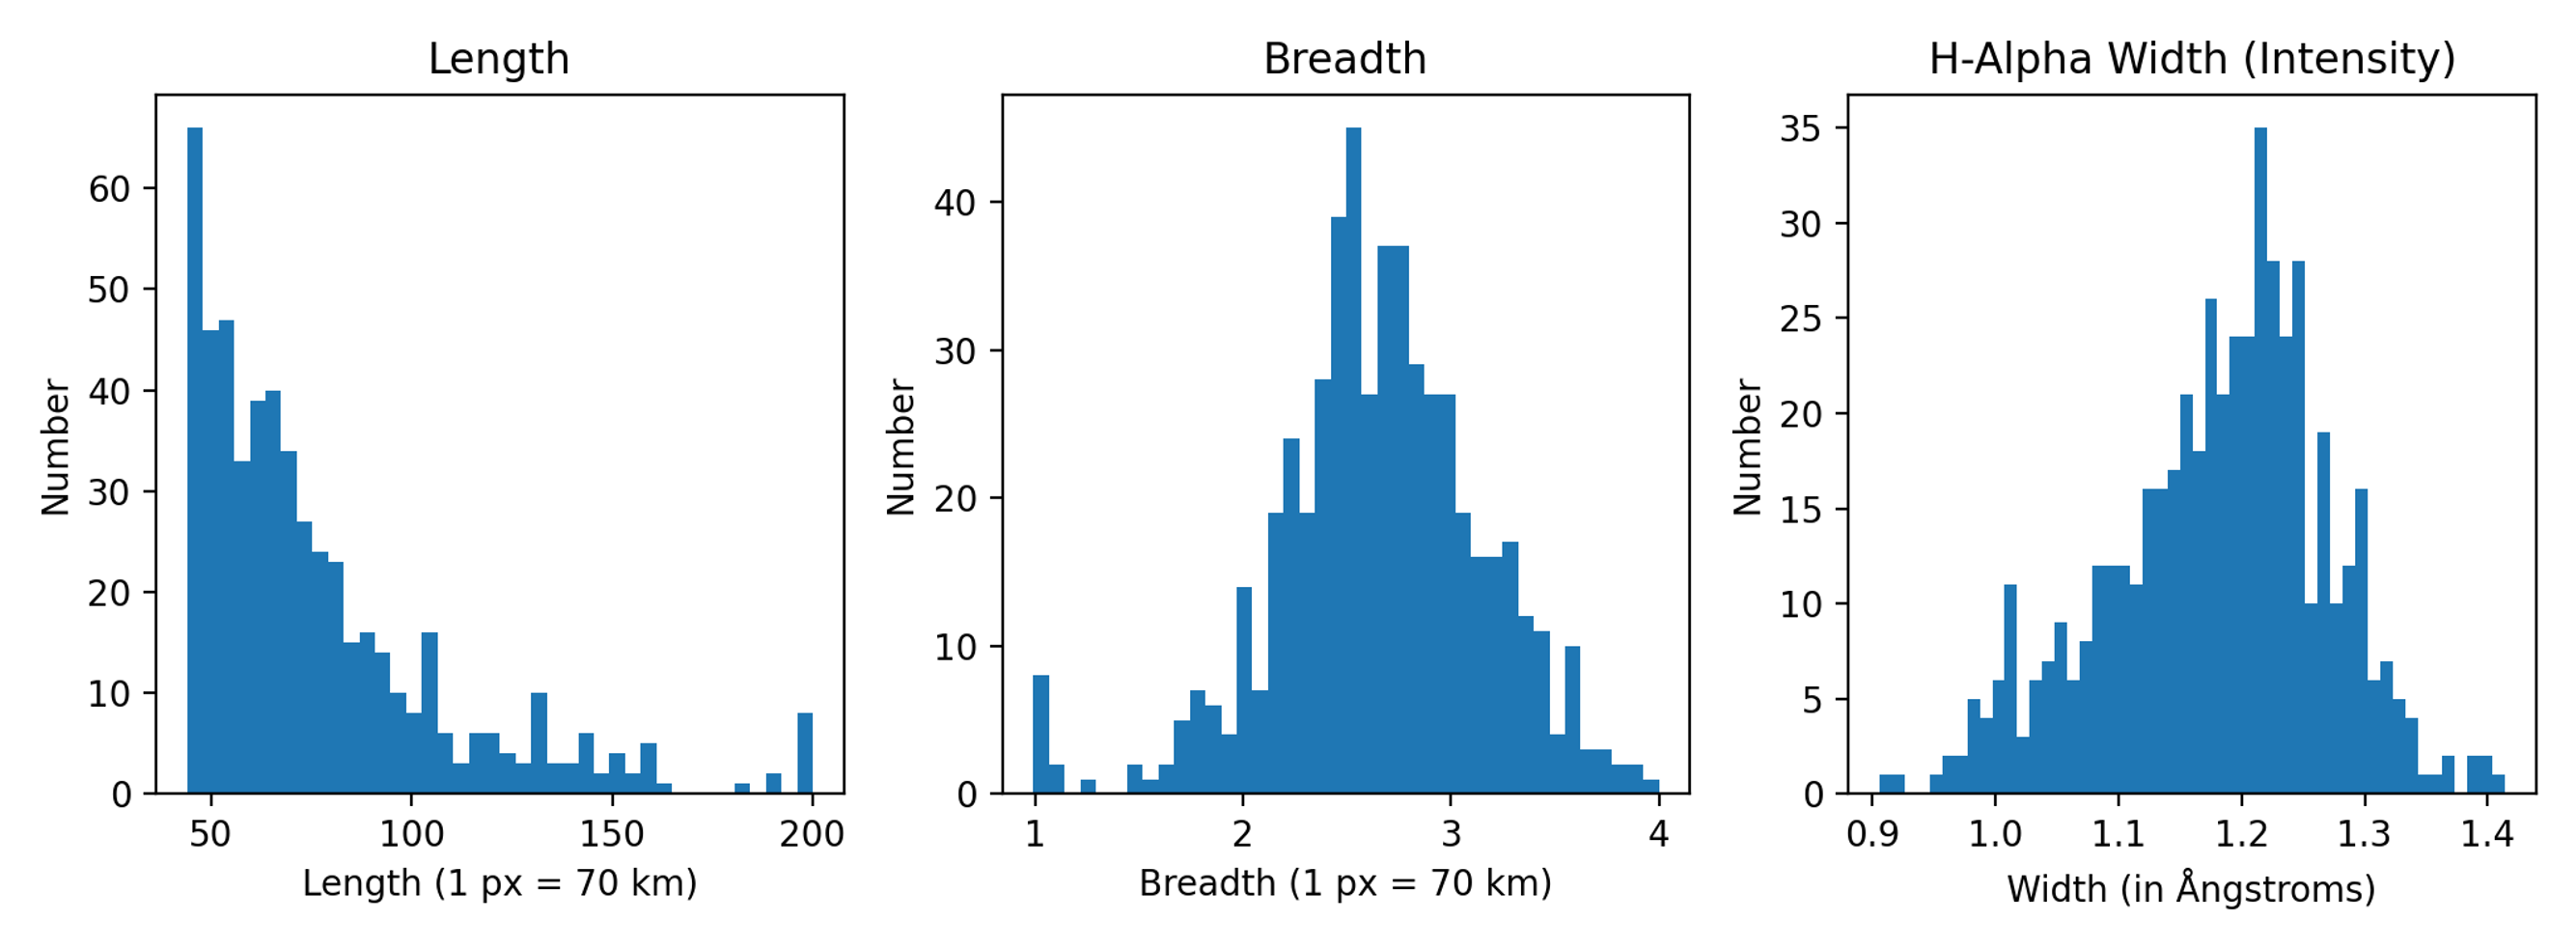
\includegraphics[width=0.9\textwidth]{results.png} 
 \caption{Left: Distribution of hot fibrils' lengths. A threshold of at least 50 pixels (3500 km) was used when selecting features. The average length of a hot fibril amounts to about 5500 km. Center: distribution of breadths. The average breadth of a hot fibril is of order 200 km, which is very close to the diffraction limit of the observations ($\approx$150 km). Right: distribution of H$\alpha$ widths. Hot fibrils have an average H$\alpha$ width of  1.18 \AA, which following \cite{2019ApJ...881...99M} would correspond to an approximate temperature of over 10,000 K.} \label{fig_results}
\end{center}
\end{figure}


\section {Conclusions} 

We analyzed the spatial characteristics of the spectral width of H$\alpha$, a quantity correlated with local T$_e$, in a plage region. To this end we have successfully adapted the OCCULT-2 algorithm, originally developed to trace coronal loops \citep{2013Entrp..15.3007A}, to identifiy curvilinear features at high spatial resolution. We find 
over 500 ``hot fibrils'' (i.e. features with a large H$\alpha$ spectral width) in our 96'' $\times$ 96'' FOV, with a suggested temperatures in excess of 10,000 K, i.e. significantly hotter than the average chromosphere. 

These features have an average length of around 5,500 km, and, while their general orientation is the same 
as for intensity features, their extension does not cover the whole FOV. This suggests that the heating events causing the large spectral widths occur only in 
a fraction of the fibrils as typically identified in the core of chromospheric lines, and, in particular, the heating occurs in the portion closer to their magnetic footpoints. 
Finally, their ``breadth'' (transversal extension) is of only 200 km, which indicates that these features are probably still under-resolved. Given these characteristics, and in particular the large aspect ratio of the hot fibrils, Ohmic dissipation of current sheets in the chromosphere appears a probable mechanism for the heating. However, a firmer interpretation will need an analysis of the temporal evolution of the heating, over multiple solar scenes. 


\begin{acknowledgments}
\noindent
P.L. was supported by the National Science Foundation REU program, award \#1659878. G.C. acknowledges a IAU travel grant for participation in the General Assembly. The National Solar Observatory is operated by the Association of Universities for Research in Astronomy, Inc. (AURA),
under cooperative agreement with the National Science Foundation. We are extremely grateful to the Local Organizing Committee for the organization of an excellent  Assembly in spite of the many logistical difficulties.  \end{acknowledgments}

%\section{Bibliography}

%Alternatively, one can use natbib linking to their own bibtex library. You will need the aa.bst file in your directory
%%
\bibliographystyle{aa}
\bibliography{fibril_biblio.bib}
\end{document}


***** from here, some old stuff ****


Now the bibliography. CPU traditionally uses the:

\begin{verbatim}

\begin{thebibliography}{} ; 

\bibitem[] ; 

\end{thebibliography} 
 
 \end{verbatim}
 
\noindent set of commands, but if you prefer, you can use 
natbib linking to your own bibtex library. In this case do not forget to upload your bibtex library with all the source files. 


%Definition of a few common journal names 
\def\apj{{ApJ}}    
\def\nat{{Nature}}    
\def\jgr{{JGR}}    
\def\apjl{{ApJL}}    
\def\aap{{A\&A}}   
\def\mnras{{MNRAS}}
\def\aj{{AJ}}
\let\mnrasl=\mnras
\def\hia{{Highlights of Astronomy}}
\def\solphys{{Solar Physics}}
\def\ssr{{Space Science Reviews}}
\def\apjs{{ApJS}}
\def\araa{{ARA\&A}}



%\begin{thebibliography}{}
%\bibitem[{Cauzzi} {et~al.}(2015)]{2015HiA....16..439C}
%{Cauzzi}, G., {Tritschler}, A., \& {Deng}, Y., 2015, \hia, 16, 439
%\bibitem[{Cauzzi} {et~al.}(2009)]{2009A&A...503..577C}
%{Cauzzi}, G., {Reardon}, K., {Rutten}, R.J., {Tritschler}, A., \& {Uitenbroek}, H., 2009, \aap, 503, 577
%\end{thebibliography}


